\documentclass[10pt, a4paper]{article}
\usepackage{lrec}
\usepackage{multibib}
\newcites{languageresource}{Language Resources}
\usepackage{graphicx}
\usepackage{tabularx}
\usepackage{soul}
\usepackage{amssymb}
% for eps graphics

\usepackage{epstopdf}
\usepackage[latin1]{inputenc}

\usepackage{hyperref}
\usepackage{xstring}

\newcommand{\secref}[1]{\StrSubstitute{\getrefnumber{#1}}{.}{ }}

\title{Evaluation of Croatian Word Embeddings\\ }

\name{Luk�\v{s} Svoboda, Slobodan Beliga}

\address{Department of Computer Science and Engineering, Faculty of Applied Sciences, University of West Bohemia, Affiliation2, Affiliation3 \\
         Univerzitn\'{i} 8, 306 14 Plze\v{n}, Czech Republic, Address2, Address3 \\
         svobikl@kiv.zcu.cz, sbeliga@uniri.hr\\
}        


\abstract{
Many unsupervised learning techniques have been investigated to obtain useful word embedding representation. Research is focusing mostly on English and less on highly inflected languages from Slavic family.\\
We derived new corpus from the original \emph{Word2vec} and added some of the specific linguistic aspect from Croatian language. 
We compared two popular word representation models, \emph{Word2Vec} and \emph{Glove}. Models has been trained on a new robust Croatian analogy corpus. We also translated WordSim353 and RG64 corpuses to Croatian and made basic semantic measurements.\\
Results show that models are able to create meaningful word representation, however this research has shown that free word order and the higher morphological complexity of Croatian language influences the quality of resulting word embeddings.
}

\begin{document}

\maketitleabstract

\section{Introduction}

Word representation based on distributional semantics \cite{bibid}, commonly referred to as word embeddings, represent words as vectors of real numbers from low-dimensional space. The goal of such representation is to capture syntactic and semantic relationship between words. 

It was shown that the word vectors can be used for significant improving and simplifying of many NLP applications \cite{Collobert08aunified,DBLP:journals/corr/abs-1103-0398}. There are also NLP applications, where word embeddings does not help much \cite{Andreas:2014}. 

Many methods have been proposed to learn such word vector representations \cite{}. Word embedding methods Word2Vec \cite{mikolov2013efficient} and GloVe \cite{pennington2014glove} significantly outperform other methods for word embeddings. Word representations made by these methods have been successfully adapted on variety of core NLP tasks.

Most of work is focused on English. Recently the community has realized that the research should focus on other languages with rich morphology and different syntax \cite{it corpus, arabic corpus}, but there is still little attention to highly inflected languages from Slavic family. These languages are highly inflected and have a relatively free word order.

In this paper, we focus on Croatian word embeddings. To be able to compare different word embeddings methods, we created two dataset based on original WordSim353\cite{bibid} and RG64\cite{bibid} translated to Croatian.
Except the similarity between words, we would like to explore other semantic and syntactic properties hidden in word embeddings. A new evaluation scheme based on word analogies were presented in \cite{mikolov2013efficient}.
Based on this popular evaluation scheme, we have produced a Croatian version of original Word2Vec analogy corpus in order to qualitatively compare the performance of different models. 





\section{Related Work}
Nowadays, word embeddings  are typically obtained as a product of training neural network-based language models. Language modeling is a classical NLP task of predicting the probability distribution over the "next" word. In these models a word embedding is a vector in $ \mathbb{R}^{n}	$, with the value of each dimension being a feature that weights the relation of the word with a "latent" aspect of the language. These features are jointly learned from plain unannotated text data. This principle is known as the \textit{distributional hypothesis}. The direct implication of this hypothesis is that the word meaning is related to the context where it usually occurs and thus it is possible to compare the meanings of two words by statistical comparisons of their contexts. This implication was confirmed by empirical tests carried out on human groups in \cite{RubensteinGoodenough65,Charles2000}. 

There is a variety of datasets for measuring semantic relatedness between English words, such as \emph{WordSimilarity-353} \cite{ws353}, \emph{Rubenstein and Goodenough (RG)} \cite{RubensteinGoodenough65}, \emph{Rare-words} \cite{Luong-etal:conll13:morpho}, \emph{Word pair similarity in context} \cite{Huang:2012:IWR:2390524.2390645}, and many others. Evaluation scheme based on word analogies were presented in \cite{mikolov2013efficient}.

To the best of our knowledge, only small portion of recent studies attempted evaluating Croatian word embeddings. In  \cite{neural network cr article} authors translated a few questions from English analogy corpus to Croatian to be able to evaluate their Neural based model. However this translation was only made for a total of 350 questions. They used it only for their own simple tests and also did not publish such a small corpus.
There is only one analogy corpus representing Slavic family language - Czech word analogy corpus presented in \cite{DBLPSvobodaB16}. 

\section{Models}
We experimented with state-of-the-art models used for generating word embeddings. Neural network based models CBOW and Skipgram from Word2Vec \cite{mikolov2013efficient} tool and model GloVe that focuses more on the global statistics of the trained data. We have also tested the most recent Fast-Text tool that promises better score for morphologically rich languages.

\subsection{CBOW} \label{sec:cbow}
CBOW (Continuous Bag-of-Words) \cite{mikolov2013efficient} tries to predict the current word according to the small context window around the word. The architecture is similar to the feed-forward NNLP (Neural Network Language Model) which has been proposed in \cite{bengio2006neural}. The NNLM is computationally expensive between the projection and the hidden layer. Thus, CBOW proposed architecture, where the (non-linear) hidden layer is removed and projection layer is shared between all words. The word order in the context does not influence the projection (see Figure \ref{fig:cbow}). This architecture also proved low computational complexity.

\subsection{Skip-gram} \label{sec:skip}
Skip-gram architecture is similar to CBOW. Although instead of predicting the current word based on the context, it tries to predict a words context based on the word itself \cite{mikolov2013distributed}. Thus, intention of the Skip-gram model is to find word patterns that are useful for predicting the surrounding words within a certain range in a sentence  (see Figure \ref{fig:skip}). Skip-gram model estimates the syntactic properties of words slightly worse than the CBOW model, but it is much better for modeling the word semantics on English test set \cite{mikolov2013efficient} \cite{mikolov2013distributed}. Training of the Skipgram model does not involve dense matrix multiplications \ref{fig:skip} and that makes training also extremely efficient \cite{mikolov2013distributed}.

\subsection{GloVe}
GloVe (Global Vectors) \cite{pennington2014glove} model focuses more on the global statistics of the trained data. The main concept of this model is the observation that ratios of word-word co-occurrence probabilities have the potential for encoding meaning of words. This approach sequentially analyzes word contexts iterating on word windows across the corpus. The authors define $ P_{ij} = p(j|i) $ as the probability that the word $ w_j $ appears in the context of word $ w_i $. The authors

\subsection{Fast-Text}
FastText\cite{bojanowski2016enriching} combines concepts of CBOW (resp. Skip-Gram) architectures introduced earlier in Section \ref{sec:cbow} and \ref{sec:skip}. These include representing sentences with bag of words and bag of n-grams, as well as using subword information, and sharing information across classes through a hidden representation. 

 
\subsection{Training data}
We trained our models on two datasets in the Croatian language. We made the entire dump of Croatian Wikipedia (dated 08-2017) and ... 

Fo
One Billion Word Benchmark \cite{DBLPChelbaMSGBK13}

Number of documents, 
\begin{table}[!h]
	\begin{center}
		\begin{tabularx}{\columnwidth}{|l|X|X|X|}
			
			\hline
			&Vocabulary&Vocabulary tf>5&Tokens\\
			\hline
			EN corpus& 793,471& & 829,250,940\\
			CR WIKI& 793,471& & 829,250,940\\
			\hline
			
		\end{tabularx}
		\caption{The caption of the table}
	\end{center}
\end{table}

\subsection{Parameters}



\section{Corpus}
Original Word2Vec analogy  corpus is composed by 19,558 questions divided in two tested group : semantic and syntactic questions, e.g. king : man = woman : queen. Fourth word in question is typically predicted one). 
\begin{table}[!h]
	\begin{center}
		\begin{tabularx}{\columnwidth}{|l|X|}
			
			\hline
			Level&Tools\\
			\hline
			Morphology & Pitrat Analyser\\
			\hline
			Syntax & LFG Analyser (C-Structure)\\
			\hline
			Semantics & LFG F-Structures + Sowa's\\
			& Conceptual Graphs\\
			\hline
			
		\end{tabularx}
		\caption{The caption of the table}
	\end{center}
\end{table}

\section{Experiments}

\begin{table}[!h]
	\begin{center}
		\begin{tabularx}{\columnwidth}{|l|X|}
			
			\hline
			Level&Tools\\
			\hline
			Morphology & Pitrat Analyser\\
			\hline
			Syntax & LFG Analyser (C-Structure)\\
			\hline
			Semantics & LFG F-Structures + Sowa's\\
			& Conceptual Graphs\\
			\hline
			
		\end{tabularx}
		\caption{Syntactic questions}
	\end{center}
\end{table}


\begin{table}[!h]
	\begin{center}
		\begin{tabularx}{\columnwidth}{|l|X|}
			
			\hline
			Level&Tools\\
			\hline
			Morphology & Pitrat Analyser\\
			\hline
			Syntax & LFG Analyser (C-Structure)\\
			\hline
			Semantics & LFG F-Structures + Sowa's\\
			& Conceptual Graphs\\
			\hline
			
		\end{tabularx}
		\caption{Semantic questions}
	\end{center}
\end{table}

\begin{table}[!h]
	\begin{center}
		\begin{tabularx}{\columnwidth}{|l|X|}
			
			\hline
			Level&Tools\\
			\hline
			Morphology & Pitrat Analyser\\
			\hline
			Syntax & LFG Analyser (C-Structure)\\
			\hline
			Semantics & LFG F-Structures + Sowa's\\
			& Conceptual Graphs\\
			\hline
			
		\end{tabularx}
		\caption{Total score}
	\end{center}
\end{table}

\section{Conclusion}

\section{Page Numbering}

\textbf{Please do not include page numbers in your article.} The definitive page
numbering of articles published in the proceedings will be decided by the
organising committee.

\section{Headings / Level 1 Headings}

Headings should be capitalised in the same way as the main title, and centred
within the column. The font used is Times New Roman 12 bold. There should
also be a space of 12 pt between the title and the preceding section, and
a space of 3 pt between the title and the text following it.

\subsection{Level 2 Headings}

The format for level 2 headings is the same as for level 1 Headings, with the
font Times New Roman 11, and the heading is justified to the left of the column.
There should also be a space of 6 pt between the title and the preceding
section, and a space of 3 pt between the title and the text following it.

\subsubsection{Level 3 Headings}

The format for level 3 headings is the same as for level 2 headings, except that
the font is Times New Roman 10, and there should be no space left between the
heading and the text. There should also be a space of 6 pt between the title and
the preceding section, and a space of 3 pt between the title and the text
following it.

%\subsubsection{Example of a sub-subsection with a long heading that will occupy two lines}
%
%Yet another example of a sub-subsection. Yet another example of a sub-subsection. Yet another example of a sub-subsection. Yet another example of a sub-subsection. Yet another example of a sub-subsection.

\section{Citing References in the Text}

\subsection{Bibliographical References}

All bibliographical references within the text should be put in between
parentheses with the author's surname followed by a comma before the date
of publication \cite{Martin-90}. If the sentence already includes the author's
name, then it is only necessary to put the date in parentheses:
\newcite{Martin-90}. When several authors are cited, those references should be
separated with a semicolon: \cite{Martin-90,CastorPollux-92}. When the reference
has more than three authors, only cite the name of the first author followed by
``et al.'' (e.g. \cite{Superman-Batman-Catwoman-Spiderman-00}).

\subsection{Language Resource References}

\subsubsection{When Citing Language Resources}

When citing language resources, we recommend to proceed in the same way to
bibliographical references, except that, in order to make them appear in
a separate section, you need to use the \texttt{\\citelanguageresource} tag.
Thus, a language resource should be cited as \citelanguageresource{speecon}.


\subsubsection{When Not Citing Any Language Resource}

When no language resource needs to be cited in the paper, you need to comment
out a few lines in the \texttt{.tex} file:

\begin{verbatim}
% \usepackage{multibib}
% \newcites{languageresource}{}
% \section{Language Resource References}
% \bibliographystylelanguageresource
%   {lrec}
% \bibliographylanguageresource{xample}
\end{verbatim}

\section{Figures \& Tables}
\subsection{Figures}

All figures should be centred and clearly distinguishable. They should never be
drawn by hand, and the lines must be very dark in order to ensure a high-quality
printed version. Figures should be numbered in the text, and have a caption in
Times New Roman 10 pt underneath. A space must be left between each figure and
its respective caption. 

Example of a figure enclosed in a box:

\begin{figure}[!h]
\begin{center}
%\fbox{\parbox{6cm}{
%This is a figure with a caption.}}
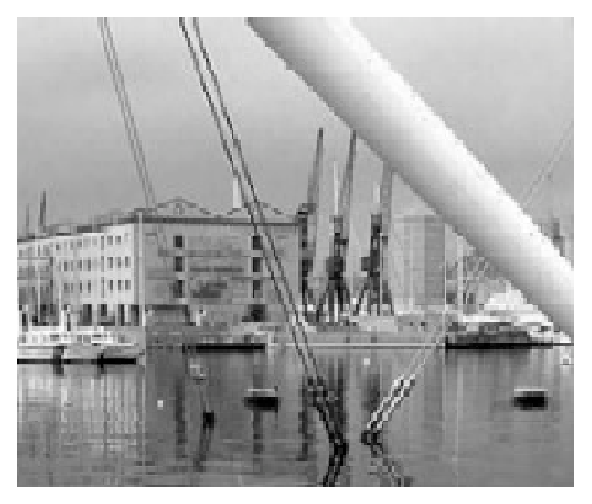
\includegraphics[scale=0.5]{image1.eps} 
\caption{The caption of the figure.}
\label{fig.1}
\end{center}
\end{figure}

Figure and caption should always appear together on the same page. Large figures
can be centred, using a full page.
%NB: an example of large figures is missing.  \newpage

\subsection{Tables}

The instructions for tables are the same as for figures.
%Two types of tables are distinguished: in-column and big tables that don't fit in the columns.
%\subsection{In-column tables}
%An example of an in-column table is presented here.
%


%\subsection{Big tables}
%
%An example of a big table which extends beyond the column and will
%float in the next page.
%
% \begin{table*}[ht]
% \begin{center}
% \begin{tabular}{|l|l|}
%
%       \hline
%       Level&Tools\\
%       \hline\hline
%       Morphology & Pitrat Analyser\\
%       Syntax & LFG Analyser (C-Structure)\\
%       Semantics & LFG F-Structures + Sowa's Conceptual Graphs  \\
%       \hline
%
% \end{tabular}
% \caption{The caption of the big table}
% \end{center}
% \end{table*}
%

\section{Footnotes}

Footnotes are indicated within the text by a number in
superscript\footnote{Footnotes should be in Times New Roman 9 pt, and appear at
the bottom of the same page as their corresponding number. Footnotes should also
be separated from the rest of the text by a horizontal line 5 cm long.}.

\section{Copyrights}

The Lan\-gua\-ge Re\-sour\-ce and Evalua\-tion Con\-fe\-rence (LREC)
proceedings are published by the European Language Resources Association (ELRA).
They are available online from the conference website.


ELRA's policy is to acquire copyright for all LREC contributions. In assigning
your copyright, you are not forfeiting your right to use your contribution
elsewhere. This you may do without seeking permission and is subject only to
normal acknowledgement to the LREC proceedings. The LREC 2018 Proceedings are
licensed under CC-BY-NC, the Creative Commons Attribution-Non-Commercial 4.0
International License.

\section{Conclusion}

Your submission of a finalised contribution for inclusion in the LREC
proceedings automatically assigns the above-mentioned copyright to ELRA.


\section{Acknowledgements}

Place all acknowledgements (including those concerning research grants and
funding) in a separate section at the end of the article.

\section{Providing References}

\subsection{Bibliographical References}
Bibliographical references should be listed in alphabetical order at the
end of the article. The title of the section, ``Bibliographical References'',
should be a level 1 heading. The first line of each bibliographical reference
should be justified to the left of the column, and the rest of the entry should
be indented by 0.35 cm.

The examples provided in Section \secref{main:ref} (some of which are fictitious
references) illustrate the basic format required for articles in conference
proceedings, books, journal articles, PhD theses, and chapters of books.

\subsection{Language Resource References}

Language resource references should be listed in alphabetical order at the end
of the article, in the \textbf{Language Resource References} section, placed after
the \textbf{Bibliographical References} section. The title of the ``Language Resource
References'' section, should be a level 1 heading. The first line of each
language resource reference should be justified to the left of the column, and
the rest of the entry should be indented by 0.35 cm. The example in Section 
\secref{lr:ref} illustrates the basic format required for language resources.

In order to be able to cite a language resource, it must be added to
the \texttt{.bib} file first, as a \texttt{@LanguageResource} item type, which
contains the following fields:

\begin{itemize}
    \item{\texttt{author}: the builder of the resource}
    \item{\texttt{title}: the name of the resource}
    \item{\texttt{publisher}: the publisher of the resource (project,
          organisation etc)}
    \item{\texttt{year}: year of the resource release}
    \item{\texttt{series}: more general resource set this language resource
          belongs to}
    \item{\texttt{edition}: version of the resource}
    \item{\texttt{islrn}: the International Standard Language Resource Number
          (ISLRN) of the resource\footnote{The ISLRN number is available from
          \texttt{http://islrn.org}}} 
\end{itemize}

If you want the full resource author name to appear in the citation, the
language resource author name should be protected by enclosing it between
\texttt{\{...\}}, as shown in the model \texttt{.bib} file.

\vspace{.3\baselineskip}

\section*{Appendix: How to Produce the \texttt{.pdf} Version}

In order to generate a PDF file out of the LaTeX file herein, when citing
language resources, the following steps need to be performed:

\begin{itemize}
    \item{Compile the \texttt{.tex} file once}
    \item{Invoke \texttt{bibtex} on the eponymous \texttt{.aux} file}
    \item{Invoke \texttt{bibtex} on the \texttt{languageresources.aux} file}
    \item{Compile the \texttt{.tex} file twice}
\end{itemize}

% \nocite{*}
\section{Bibliographical References}
\label{main:ref}

\bibliographystyle{lrec}
\bibliography{cranalogy}


\section{Language Resource References}
\label{lr:ref}
\bibliographystylelanguageresource{lrec}
\bibliographylanguageresource{cranalogy}

\end{document}
